%%---------------------------------------------------------------------------%%
%% dbs.tex
%% Thomas M. Evans
%% $Id$
%%---------------------------------------------------------------------------%%
\documentclass[11pt]{../tex/rnote}
\usepackage[centertags]{amsmath}
\usepackage{amssymb,amsthm,graphicx}
\usepackage[mathcal]{euscript}
\usepackage{tabularx}
\usepackage{cite}
\usepackage{c++}
\usepackage{tmadd,tmath}
\usepackage{stl}
\usepackage{draco_bs}
\usepackage{alltt}
\usepackage{makeidx}

%%---------------------------------------------------------------------------%%
%% DEFINE SPECIFIC ENVIRONMENTS HERE
%%---------------------------------------------------------------------------%%

\newcommand{\dsxx}{\pkg{ds\raisebox{.2ex}{\scriptsize++}}}
\newcommand{\imc}{\pkg{imc}}

\newcommand{\draco}{\sys{Draco}}

\newcommand{\autoconf}{\soft{Autoconf}}
\newcommand{\automake}{\soft{Automake}}
\newcommand{\make}{\soft{Make}}

\makeindex

%%---------------------------------------------------------------------------%%
%% BEGIN DOCUMENT
%%---------------------------------------------------------------------------%%

\begin{document}

%%---------------------------------------------------------------------------%%
%% OPTIONS FOR NOTE
%%---------------------------------------------------------------------------%%

\toms{Distribution}
%\toms{Joe Sixpak/XTM, MS B226}
\refno{X-6:97-??? (U)}
\subject{The Draco Build System}

%-------NO CHANGES
\divisionname{Computer and Computational Sciences}
\groupname{CCS--4:Transport Methods Group}
\fromms{Thomas M. Evans/CCS-4 D409}
\phone{(505)665--3677}
\originator{tme}
\typist{tme}
\date{\today}
%-------NO CHANGES

%-------OPTIONS
%\reference{NPB Star Reimbursable Project}
%\thru{P. D. Soran, XTM, MS B226}
%\enc{list}      
%\attachments{list}
%\cy{list}
%\encas
%\attachmentas
%\attachmentsas 
%-------OPTIONS

%%---------------------------------------------------------------------------%%
%% DISTRIBUTION LIST
%%---------------------------------------------------------------------------%%

\distribution {}

%%---------------------------------------------------------------------------%%
%% BEGIN NOTE
%%---------------------------------------------------------------------------%%

\opening

\begin{abstract}
  
  We present an updated build system for the \draco\ component
  library.  The \draco\ Build System (DBS) \index{Draco Build System}
  is designed to facilitate both development and usage on multiple
  platforms.  The DBS complies with the GNU Coding Standards for
  software packages.  It has been designed according to the following
  list of requirements:
  \begin{enumerate}
  \item support for simultaneous, multiple configurations;
  \item support for \C++ on all ASCI platforms;
  \item automated unit and regression testing;
  \item the ability to support multiple code projects;
  \item support for external vendors;
  \item support for multiple languages;
  \item extensibility;
  \item low-cost on developers to add new packages, code, and tests; 
  \item compliance with the GNU coding standard \cite{gnu}.
  \end{enumerate}
  These requirements are largely met by the DBS.  In fact, the DBS is
  being used as the build system for 4 CCS--4 projects.
  
  The build system uses four GNU development tools, \autoconf,
  \automake, and \make. These tools are all freely available from the
  Free Software Foundation.

\end{abstract}

%%---------------------------------------------------------------------------%%
%% INCLUDES
%%---------------------------------------------------------------------------%%

%%---------------------------------------------------------------------------%%
%% introduction for imc-dev manual
%%---------------------------------------------------------------------------%%

\section{Introduction}

The \imctest\ package represents a first step towards the development
of \milagro.  In this sense, \imctest\ may be considered an early
release of \milagro.  The goals of \imctest\ are:
\begin{enumerate}
\item develop an extensible \C++ object-oriented/generic design;
\item test the implementation of the IMC algorithm on several simple
  test problems;
\item test the parallel performance of IMC on several platforms.
\end{enumerate}
The object-oriented/generic design of \imctest\ will ensure an easy
transition to the full \milagro\ package.  The improvements and
additions that are required to promote \imctest\ to \milagro\ include:
\begin{enumerate}
\item interfaces to various host-codes;
\item improved physics;
\item new mesh-types and geometries;
\end{enumerate}
The classes and data structures in \imctest\ are easily extensible;
thus, the classes used in \imctest\ should work in \milagro. For more
information, the \jayenne\ code development plan is described in
detail in Ref.~\citen{xtm:rn98xxx}.

The purpose of this manual is to document the code structure of the
\imctest\ package for users of the \imctest\ library.  In essence, this
manual contains the following information:
\begin{itemize}
\item a listing and description of the classes and data structures
  which comprise the \imctest\ library;
\item descriptions of the interactions between classes and types in
  \imctest;
\item descriptions of the interfaces for each class in \imctest.
\end{itemize}
The information presented herein will facilitate easy usage of the
\imctest\ library by code developers in X-division.  It will also serve
as a reference for users of the code.


%%---------------------------------------------------------------------------%%
%% model.tex 
%% description of the draco component library and overview of the build system
%% ---------------------------------------------------------------------------%%

\chapter{The Draco Model}
\label{chap:model}

This chapter presents an overview of the \draco\ build model, architecture and
source.  We present, in detail, the requirements for the \draco\ build
system in \S~\ref{sec:build_sys_req}.  Because the \draco\ build model
was originally designed to conform to the GNU coding standard, a brief
summary of GNU requirements is given in \S~\ref{sec:gnu_build_model}.
Finally, this chapter concludes with a description of the \draco\ 
source tree and files that are created during configuring and
building.

%%---------------------------------------------------------------------------%%

\section{Overview of Draco}
\label{sec:overview_of_draco}

Documentation describing the purpose and capabilities of packages
within \draco\ is beyond the scope of this text.  However, a brief
summary of \draco\ is pertinent to this discussion.  \draco\ is a
component library for computational radiation transport.  \draco\ is
primarily a \cpp\ library; however, other language support is not
precluded in \draco.  In particular, \draco\ has plans to support \lang{ISO\_C\_BINDING} interfacing between \cpp\ and \fortran.  A more general type of 
automatic type-interfacing between \cpp\ and \fortran~\cite{gr99} was implemented to support \sys{Dante} code, but was abandoned in favor of a simpler interface paradigm.
% Additionally, we plan to incorporate a generalized interface for
%problem input specifications using \python\ extensions.

The products of \draco\ are individual component libraries
that provide reusable services geared towards radiation transport
applications.  For example, \draco\ provides random number generators that may be used by a Monte
Carlo radiation transport solver.  \draco\ also provides access to opacity models and an angular quadrature component that can be used by deterministic radiation transport solvers.  In addition to components designed for radiation transport,
\draco\ provides several service packages including \dsxx, a data
structures library that contains numeric containers, smart pointers,
and assertions, and \cfour, a communications library, among others.

%The fundamental principle guiding code design in \draco\ is templating
%on Mesh Types (MT).  Thus, the libraries in \draco\ will work with any
%code that provides a MT with the proper services.  This allows highly
%efficient implementations of various meshes to be included in generic
%radiation transport packages.  

\draco\ is designed using object-oriented~\cite{me97} \index{object-oriented}and generic
programming~\cite{au99} \index{generic programming} philosophies.  Foremost among these notions
are levelized design \index{levelized}, Design-by-Contract$^{\text{\footnotesize TM}}$, \index{ Design-by-Contract}
and the generic concept-model idea.  Other software engineering
methods are employed for quality control including regression testing,
automatic documentation, code profiling, and design and code reviews.

  

%%---------------------------------------------------------------------------%%

\section{Overview of the Draco Build Model}
\label{sec:overview_draco}

\subsection{Software Requirements}

Originally, the \draco\ build system was designed according to the GNU coding
standard and made use of  \autoconf~\cite{autoconf},
\gmake~\cite{gmake}, and \gmfour~\cite{m4} for configuring and building components.  
In 2011, this requirement was altered as the development team chose to replace the
aging build system with a \cmake-based system~\cite{cmake}.  In addition, \draco\ version
control is performed by \svn~\cite{svn-redbean}.  

Additional software is used for performing quality control.
Regression testing is handled by \cmake's \ctest\ and \cdash\ tools.  Bugs are
tracked using \teamforge~\cite{teamforge,teamforge-lanl}.  In addition, an archived email
list is available to submit design plans and discussion between team
members.  Also, \valgrind~\cite{valgrind}, \bullseye~\cite{bullseyeweb} and \cloc~\cite{clocweb} play important roles in the
quality control process.  The build system supports
processing code and tests through \valgrind\ on all platforms for performing dynamic memory and cache analysis. It supports the use of \bullseye\ for analyzing \cpp\ code coverage metrics (function and condition/decision branch coverage) and it uses \cloc\ for tracking total lines of source code.  All of this information is collected nightly by the regression system and published on the \draco\ regression dashboard at \url{http://coder.lanl.gov/cdash}.
 
The \draco\ build system contains support for multiple language
environments.  However, the primary language in use at present is the 1998 ANSI
Standard \cpp~\cite{ansi:cpp}.  \draco\ does not currently support the 2011 ANSI \cpp\ Standard~\cite{ansi:cpp11}\index{C++ 2011} because LANL standard compiler's do not support the new standard yet.  As soon as the required compilers support the new standard, \draco\ will allow code to be written that conforms to the 2011 standard. Currently, any \cpp\ compiler that conforms to the 1998 standard will compile \draco.  Portland Group, Intel and GNU \cpp\ are regularly used for building on ASC hardware. 
Currently, there
is no \fortran\ code in \draco; although, we expect that to change in
the future.  (The build system does look for a \fortran\ compiler during the configuration step so that a compatible version of LAPACK can be located and tested with the selected linker.)
Additional languages required by \draco\ are \python\ and 
\lang{PERL}.  \draco\ expects these scripting
languages to be located in a directory that is included int he developer's \comp{PATH},
and the build system checks for this.   A suite of tools that can typeset \LaTeX\ sources is also
necessary for compiling much of the documentation that comes with \draco.
  
%   Unfortunately, the Kuck and Associates
%\cpp\ compiler, \soft{KCC}~\cite{kai}, is the only ANSI Standard
%compatible compiler on the market today.  Thus, \soft{KCC} is required
%to compile \draco\ in its entirety. \soft{KCC} is available on all
%platforms of interest to Los Alamos National Laboratory and the
%Accelerated Strategic Computing Initiative (ASCI).  

With the exception of \bullseye\ and the listed commercial compilers, all of the
aforementioned software products are freely available.  Note that \bullseye\ is mainly a
development tool and is not required to configure, build, or use
\draco.  Also note that the GNU set of compilers is freely available and using them allows \draco\ to be built without the use of any commercial software.

The build system checks for the presence of each of aforementioned software products; thus, as
long as the software is in the user's path, the configuration will
succeed.  Finally, \draco\ utilizes a number of vendor libraries,
depending upon configuration, that must be installed on the system in
which \draco\ resides.  Detail on these packages and their
configuration options is given in Chap.~\ref{chap:compile}.

\begin{table}
  \begin{center}
    \caption{Required and optional tools for configuring and building \draco.}
    \label{tab:reqtools}
    \begin{tabular}{lp{1.5in}p{1.5in}p{1.5in}}\hline\hline
    
          Tool & Required  & Recommended & Optional \\ \hline
	Configuration & \cmake-2.8.6+ & \ctest & \cdash  \\
	\cpp\ compiler & Any standards compliant \cpp\ compiler &  g++ 4.5 & Intel 10-12, PGI 11 \\
	\fortran\ compiler & optional & gfortran 4.5+ & Intel 10-12, PGI-11 \\
	Build tool & any of ... & \gmake & Eclipse CDT, XCode, Visual Studio \\
	Scripting language & \cmake & \python & \perl \\
	Version control & \svn & & \git \\
	Dynamic Analysis & optional & \valgrind & \\
	Code Coverage & optional& \bullseye & \\
	Lines-of-Code & optional & \cloc & \\
	Bug Tracking & optional & \teamforge & ChangeLog, text files, email \\
	Documentation & optional & \LaTeX\ typesetting tool, \doxygen & \\	
	\hline \hline

    \end{tabular}
  \end{center}
\end{table}



\subsection{Build System Requirements}
\label{sec:build_sys_req}

In \S~\ref{sec:purpose} the requirements that guided the development
of the \draco\ build system were summarized.  In this section, we
shall take an expanded look at the complete list of requirements.  The
list of requirements for the \draco\ build system is:
%
\begin{enumerate}
\item support for simultaneous, multiple configurations (Release, Debug, Scalar, Parallel, etc);
\item support for multiple programming languages, while preferring \lang{C} and \cpp;
\item support for \cpp\ on all current ASC platforms;
\item \lang{C} and \cpp\ coding must conform strictly to issued ISO standards~\cite{ansi:cpp} \index{ISO standard}:
\begin{enumerate}
\item \cpp 03, also known as the ISO/IEC 14882:1998 standard amended by the 2003 technical corrigendum, ISO/IEC 14882:2003;
\item \lang{C99}, also known as the ANSI C ISO/IEC 9899:1999 standard;
\end{enumerate}
\item support for multiple build project types (\soft{Makefiles}~\cite{gmake}, \soft{XCode}, \soft{Eclipse}, etc.)
\item on-demand and automated unit and regression testing; \index{regression testing}
\item support for \cdash~\cite{cmake,codercdash} presentation of regression results;
\item support for \valgrind~\cite{valgrind} dynamic analysis integrated into \cdash\ presentation; \index{valgrind}
\item the ability to support multiple code projects;
\item extensible support for external vendors; 
\item support for explicit template instantiation; \index{explicit template instantiation}
\item extensibility;
\item low-cost on developers to add new packages, code, and tests; 
\item  adoption of selected sections of the GNU coding standard~\cite{gnu} \index{GNU
    Coding Standard}.
\end{enumerate}
%
We will analyze each of these requirements in turn.  First, from a
development standpoint, having multiple configurations at the same
time is a must.  This feature is required because certain tools work
better on certain platforms.  Additionally, certain tools work better
in certain environments.  For example, we often require both scalar
and parallel versions of the code for profiling and testing.  The
\draco\ build systems allow each configuration, and the products it
produces, to exist in a unique directory.  Thus, builds are not
performed in the source code tree; they are done in a user-specified
directory.  More detail is given on multiple configurations and builds 
in \S~\ref{sec:draco_src_tree} and Chap.~\ref{chap:compile}.

% #2
\draco\ is not a single language system.  Although \draco\ is
presently composed of \cpp\ code, we expect multiple languages
(in particular \lang{Fortran}) to be supported for interfacing and numerical
optimization.  The \draco\ build system is general and is not
restricted to single language support.  Supporting multiple languages
is an essential requirement because \draco\ customers utilize many
frameworks and languages.

% #3 & #4
\cpp\ source code in \draco\ must conform to the the ISO/IEC 14882:1998 standard amended by the 2003 technical corrigendum, ISO/IEC 14882:2003. \index{ISO standard} This ensures that \cpp\ sources will 
compile by any standards compliant \cpp\ compiler.  The DBS activates many compiler warning flags for Debug builds so that developers are notified if their code deviates from the standard.  In particular, code that does not compile cleaning using ASC standard compilers on target ASC platforms must be brought into compliance or be removed from the \draco\ system.

% #5
In recent years the need to support non-command line integrated development environments, \index{integrated development environment} IDE, has become increasingly important.  With the conversion of the build system from \soft{autotools} to \cmake\ in 2011, this has become a build system requirement.  The primary build tool continues to be \soft{Makefiles} but support for the \soft{Eclipse CDT} IDE on Linux and for the \soft{XCode} IDE on OS/X is also supported.

% #6-#8
The next three requirements are aimed at \draco\ system and package
developers and are essential for developing high quality software.
%  The \draco\ build system must support \dejagnu.  
Regression and unit testing are an important part of the \draco\ quality assurance program.  \draco\ developers must have the ability to run a test suite to determine if local changes adversely impact other parts of the \draco\ system.  The daily
testing of \draco\ components also ensure that commits to
one part of the library do not adversely affect other components.  These daily tests are run on multiple platforms and may catch coding issues that only appear on specific hardware/software combinations.  The results from nightly testing must be published to the \draco\ Dashboard~\cite{codercdash} and email sent to developer who request nightly updates.  Additionally, code coverage metrics by \bullseye, dynamic analysis (via \valgrind) and lines-of-code metrics must also be collected nightly so that the time evolution of issues can be tracked and to allow the \draco\ development team the data needed to target specific improvements.  Such improvements might be the addition of unit tests so that more baseline code is checked in the nightly tests or the elimination of memory errors.

% #9
In addition to being self supportive, the \draco\ build system will be designed to be exported to other code projects.  This requirement includes the ability of other code projects to use build system scripts found in \draco\ and the ability to find and link against \draco\ code and vendor code known by by \draco.  The \sys{Capsaicin} and \sys{Jayenne} code projects both employ the \draco\ build system and also link to \draco\ component libraries.

% #10
As a suite of scientific simulation tools, \draco\ components often need to link against vendor software to provide specialized capabilities.  For example, most of \draco\ is designed to be run in parallel under MPI.  MPI is a vendor tool supported by \draco.  The build system can detect the local availability of MPI and will adjust build parameters based on the flavor and version of MPI.  For example, if MPI is not found on the local system, the build system automatically switches to \comp{SCALAR} mode and does not attempt to link libraries and executables against the MPI libraries.  While \draco\ can be built without MPI, it is assumed to be a required vendor in most cases.  The GNU Scientific Library is also considered to be a required vendor for \draco\ as it provides random number generation  features and many linear algebra functions.  Optional vendors for \draco\ include BLAS, LAPACK, ScaLAPACK, BLACS, Trilinos and xmgrace among others.  Extending the \draco\ build system to support other vendors is straight forward and transparent.

% #11
A guiding principle of the \draco\ build system is explicit template
instantiation. \index{explicit template instantiation}  We have found that this provides a  more robust
and efficient build system compared to the environment where the compiler is allowed to
instantiate template classes and functions {\it automatically}.  The essence of explicit
instantiation is that the package developer determines what templated classes
are instantiated (and when they are instantiated)~\cite{cpptemplates}.  \draco\ does not implicitly
instantiate template classes and functions.  \draco\ has rules on how
template classes and functions are explicitly instantiated.  These are
listed in Chap.~\ref{chap:adding}.  Additional information for clients
that use \draco\ class and function templates is listed in
\S~\ref{sec:using}.

% #12 - #13
Another guiding principle of the \draco\ suite of components is the concept that active features are constantly changing.  New features are regularly added to \draco\ and deprecated features are removed periodically.  It is imperative that the DBS flexibly support these changes so that the developer cost of adding or removing components remain low.   This is accomplished through the encapsulation paradigm and the levelized component design of \draco.  The DBS itself must remain extensible as new requirements for the build system come into play.

% #14

The final requirement is that the \draco\ build system should continue to adhere to the GNU Coding Standard~\cite{gnu} as much as is reasonable.  Obviously, the adoption of \cmake\ and non-Makefile based build systems is not supported by this standard and we have made a deliberate decision to make the build system more flexible at the cost of standardization.  By formalizing our build model on an accepted standard, we reduce the overhead associated with maintaining the system. In the case of the \cmake-based build system, we make heavy use of the features provided by \cmake\ and avoid the use of custom build scripts except for cases that are absolutely necessary (i.e.: python scripts for running application codes and checking the results against gold standards).  A summary of the pertinent parts of the GNU standard is given in \S~\ref{sec:gnu_build_model}

\subsection{The GNU Build Model}
\label{sec:gnu_build_model}

A full description of the GNU Coding Standards is beyond the scope of
this text.  Interested readers are referred to Ref.~\cite{gnu} for
more information.  However, a brief summary of the pertinent aspects
of the coding standard is useful here.  As we have previously
mentioned, the \draco\ build system corresponds to the guidelines set
forth in the GNU standard.  The relevant parts of the GNU standard
that affect \draco\ are the sections pertaining to documentation and
program release.  We shall look at these in turn.

The GNU standard specifies the following requirements on release
documentation:
\begin{enumerate}
\item provide a manual describing the system using \soft{texinfo}, this can refer to other documentation;
% \item a \comp{NEWS} file should contain highlighted, version update information;
\item a \comp{ChangeLog} file should contain a log of changes made to the product between different releases;
\item man pages are optional.
\end{enumerate}
\draco\ does not presently have man pages, and no attempts are
underway to make them.  The other requirements are met with the
following exceptions: \draco\ uses \LaTeX\ and \doxygen\ for its documents and
contains more than one manual due to its size and multiple uses.

\subsection{The CMake Build Model}
\label{sec:cmake_build_model}

The GNU standard specifies many constraints on build and make systems including a mandate to use  \comp{configure*} scripts and standardized configure options and \comp{Makefile} targets.  The \cmake-based \draco\ build system no longer makes any attempt to support these requirements.  Instead, the following build system features must be supported:
\begin{enumerate}
\item \cmake\ will be used to configure code products;
\item Each directory in the build system will have a \comp{CMakeLists.txt} file that describes local build targets, platform checks, and local testing instructions.
\item \cmake\ guarantees certain names (e.g.: \comp{PROJECT\_NAME}, \comp{PROJECT\_BINARY\_DIR}, \comp{CMAKE\_<LANG>\_FLAGS, \comp{MPI\_FOUND}, etc.}) to exist in the build.  A more complete list can be obtained by running '\comp{cmake --help-variable-list}.'
\item \cmake\ guarantees certain build project targets will be defined:
\begin{itemize}
\item all - generate all normal targets
\item clean - remove generated files (libraries, object files, binaries, etc.)
\item Experimental - run the build and tests and submit the results to the dashboard.
\item install - copy built files to the \comp{CMAKE\_INSTALL\_PREFIX} directory 
\item test -  run the unit tests
\item uninstall - remove files copied as a result of the install target
\end{itemize}
\item The DBS standardizes additional Makefile targets:
\begin{itemize}
\item Lib\_$<$component$>$
\item  Lib\_$<$component$>$\_test
\item Ut\_$<$component$>$\_$<$testname$>$\_exe
\end{itemize}
\end{enumerate}
Because \cmake\ does not restrict the build project to \soft{Makefiles}, we don't speak explicitly about {\it Makefile targets} and instead use the term {\it build targets}.  In general, the \draco\ build system attempts to use the same variable naming conventions as \cmake.

%\begin{enumerate}
%\item \comp{configure*} scripts should be used to configure code products;
%\item hardware and software options should be controlled by the
%  \comp{--with-\textsl{feature}} or \comp{--enable-\textsl{feature}}
%  command-line specifications to \comp{configure*};
%\item standard makefile services and targets are defined.
%\end{enumerate}
%Because \draco\ uses \autoconf\ to produce \comp{configure*} scripts,
%the first two requirements are met by default.  With regard to
%makefiles, the GNU standard specifies a lengthy list of required
%targets, definitions, and acceptable utilities.  \draco\ meets all of
%these requirements.  The one exception is that \draco\ is primarily a
%\cpp\ system.  This would seem to be in violation of the GNU standard.
%However, because of the specificity of the \draco\ client base, we are
%justified in using \cpp\ as described in \S~3.4 of the GNU Coding
%Standard.

%%---------------------------------------------------------------------------%%

\section{The Draco Source Code Tree}
\label{sec:draco_src_tree}

\subsection{Draco Source Tree}

In this section we give an overview of the \draco\ source tree. The
\draco\ source tree is illustrated in Fig.~\ref{fig:src_draco}.  The
subdirectories are in \index{source tree}
\begin{figure}
  \centerline{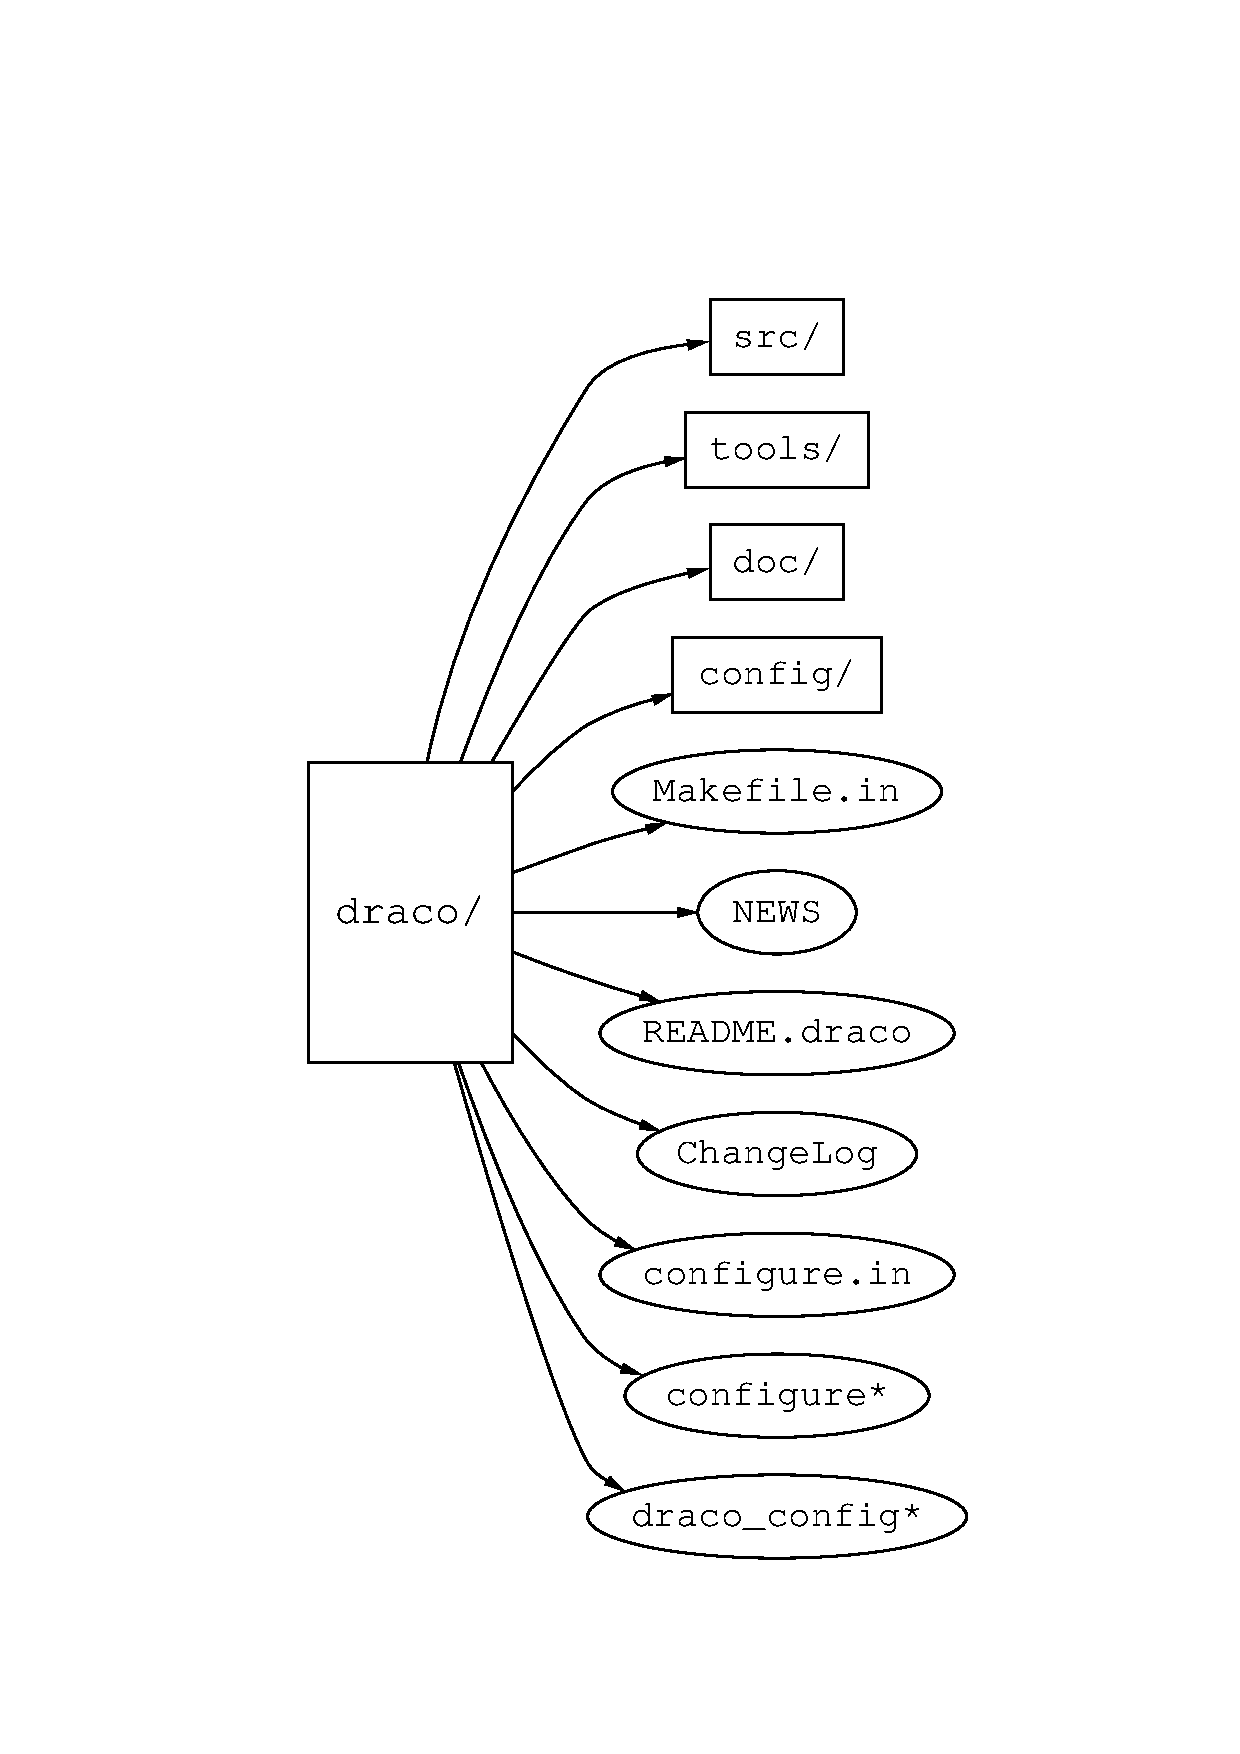
\includegraphics[clip,trim=1cm 4cm 1cm 4cm,width=3.5in]{fig/src_draco}} % [width=2in]
  \caption{The \draco\ source tree.  Directories are in boxes and
    files are in ellipses.  The subdirectories are shown in
    Fig.~\ref{fig:subdraco}.}
  \label{fig:src_draco}
\end{figure}
Figs.~\ref{fig:subdraco}a through c.  Note that these figures show the
\begin{figure}
  \begin{center}
    \begin{tabular}{ccc} 
      \subfloat[\comp{src/}]{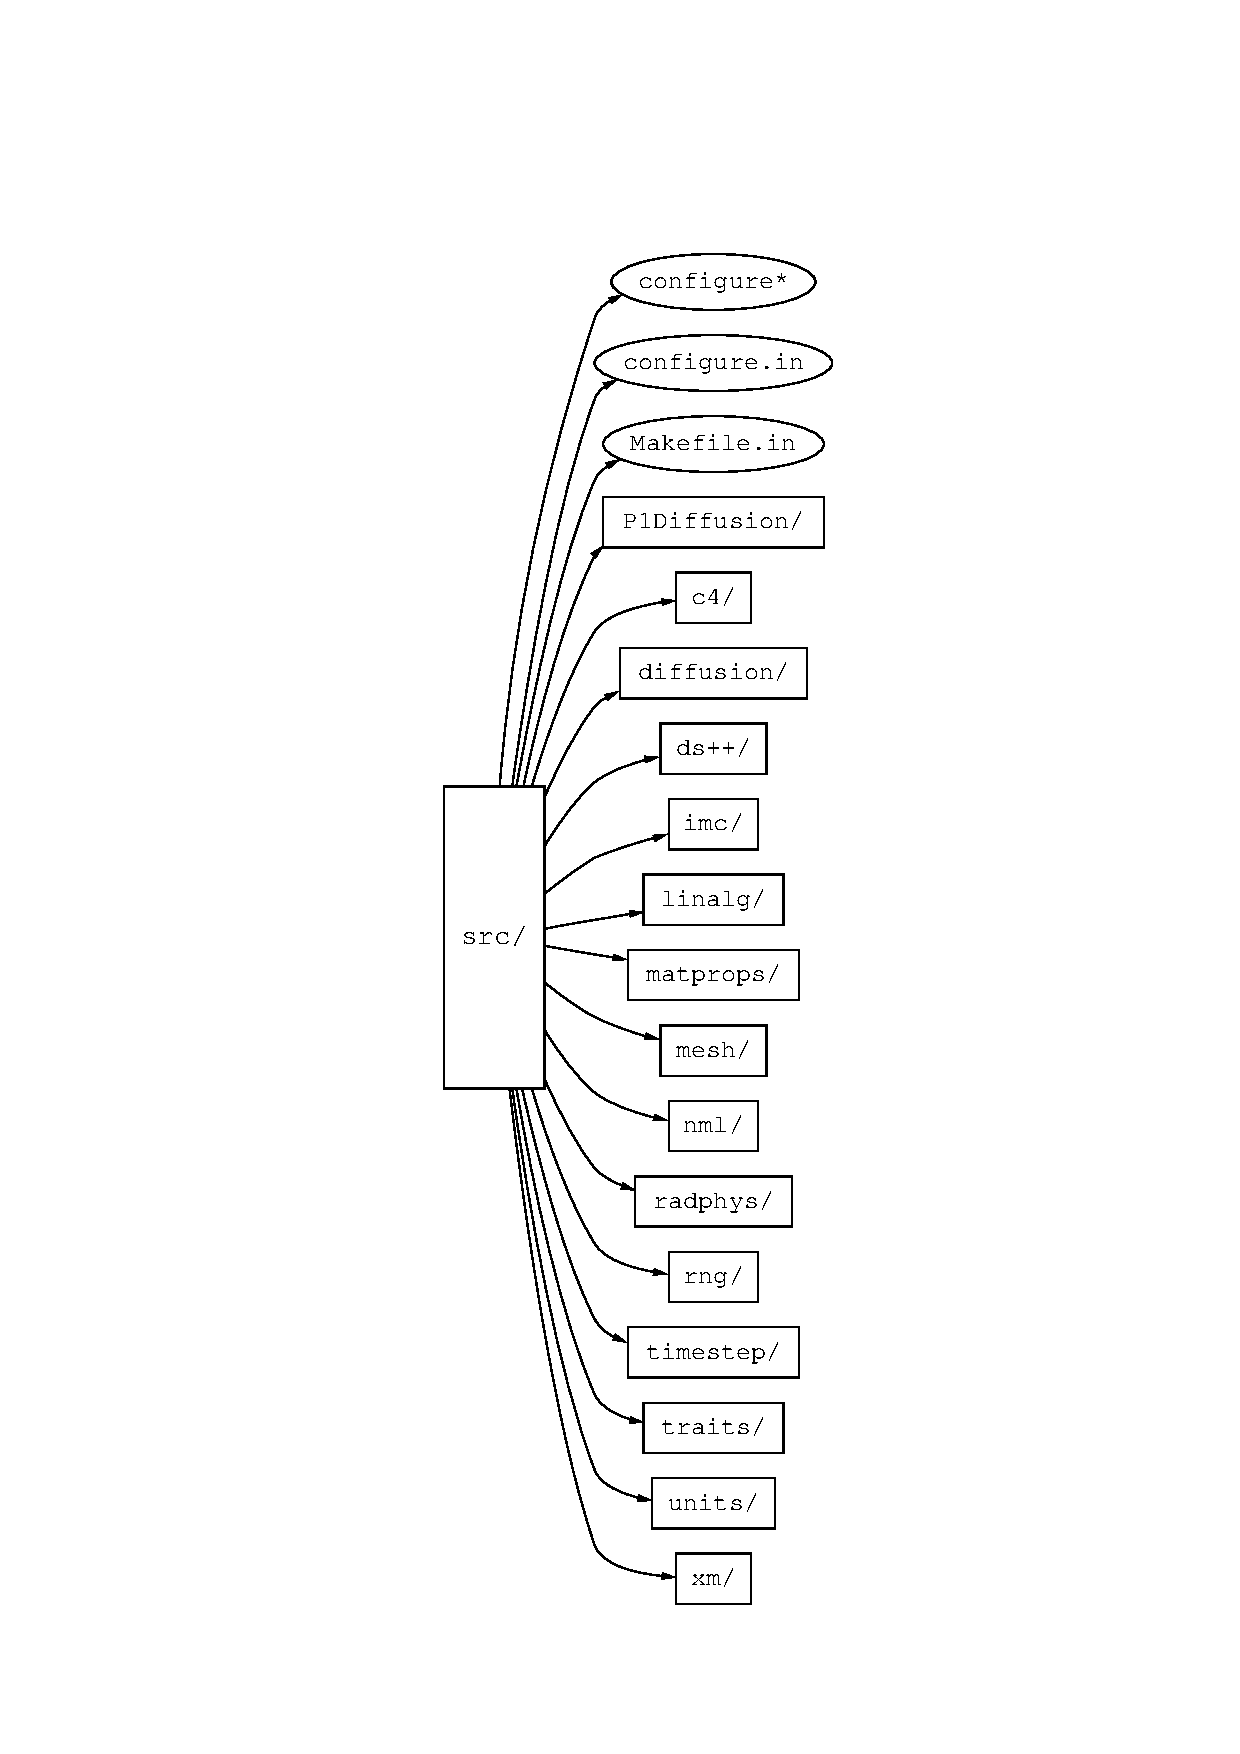
\includegraphics[clip,trim=12cm 2cm 5cm 0cm,width=1.3in]{fig/src_src}} & % trim=l b r t
      \subfloat[\comp{doc/}]{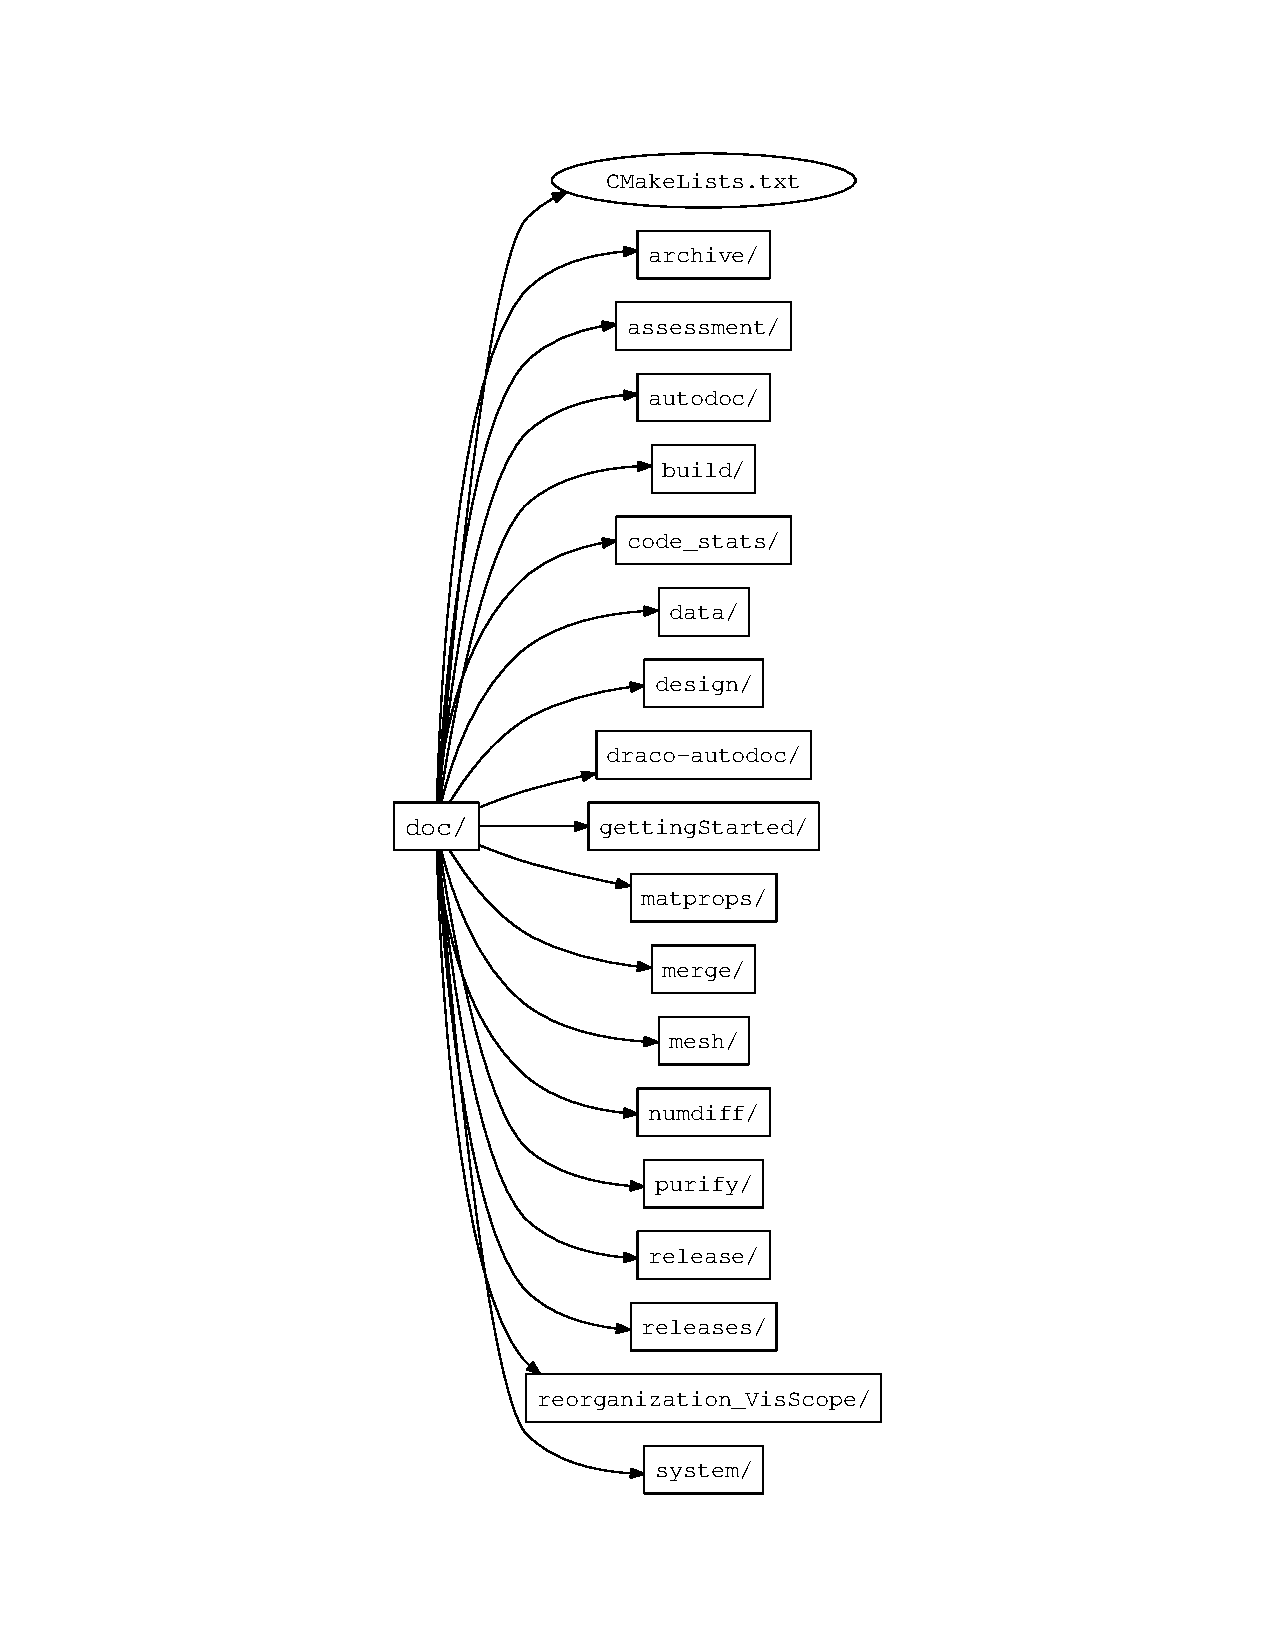
\includegraphics[clip,trim=9cm 1cm 8cm 0cm,width=1.0in]{fig/src_doc}} &
      \subfloat[\comp{config/}]{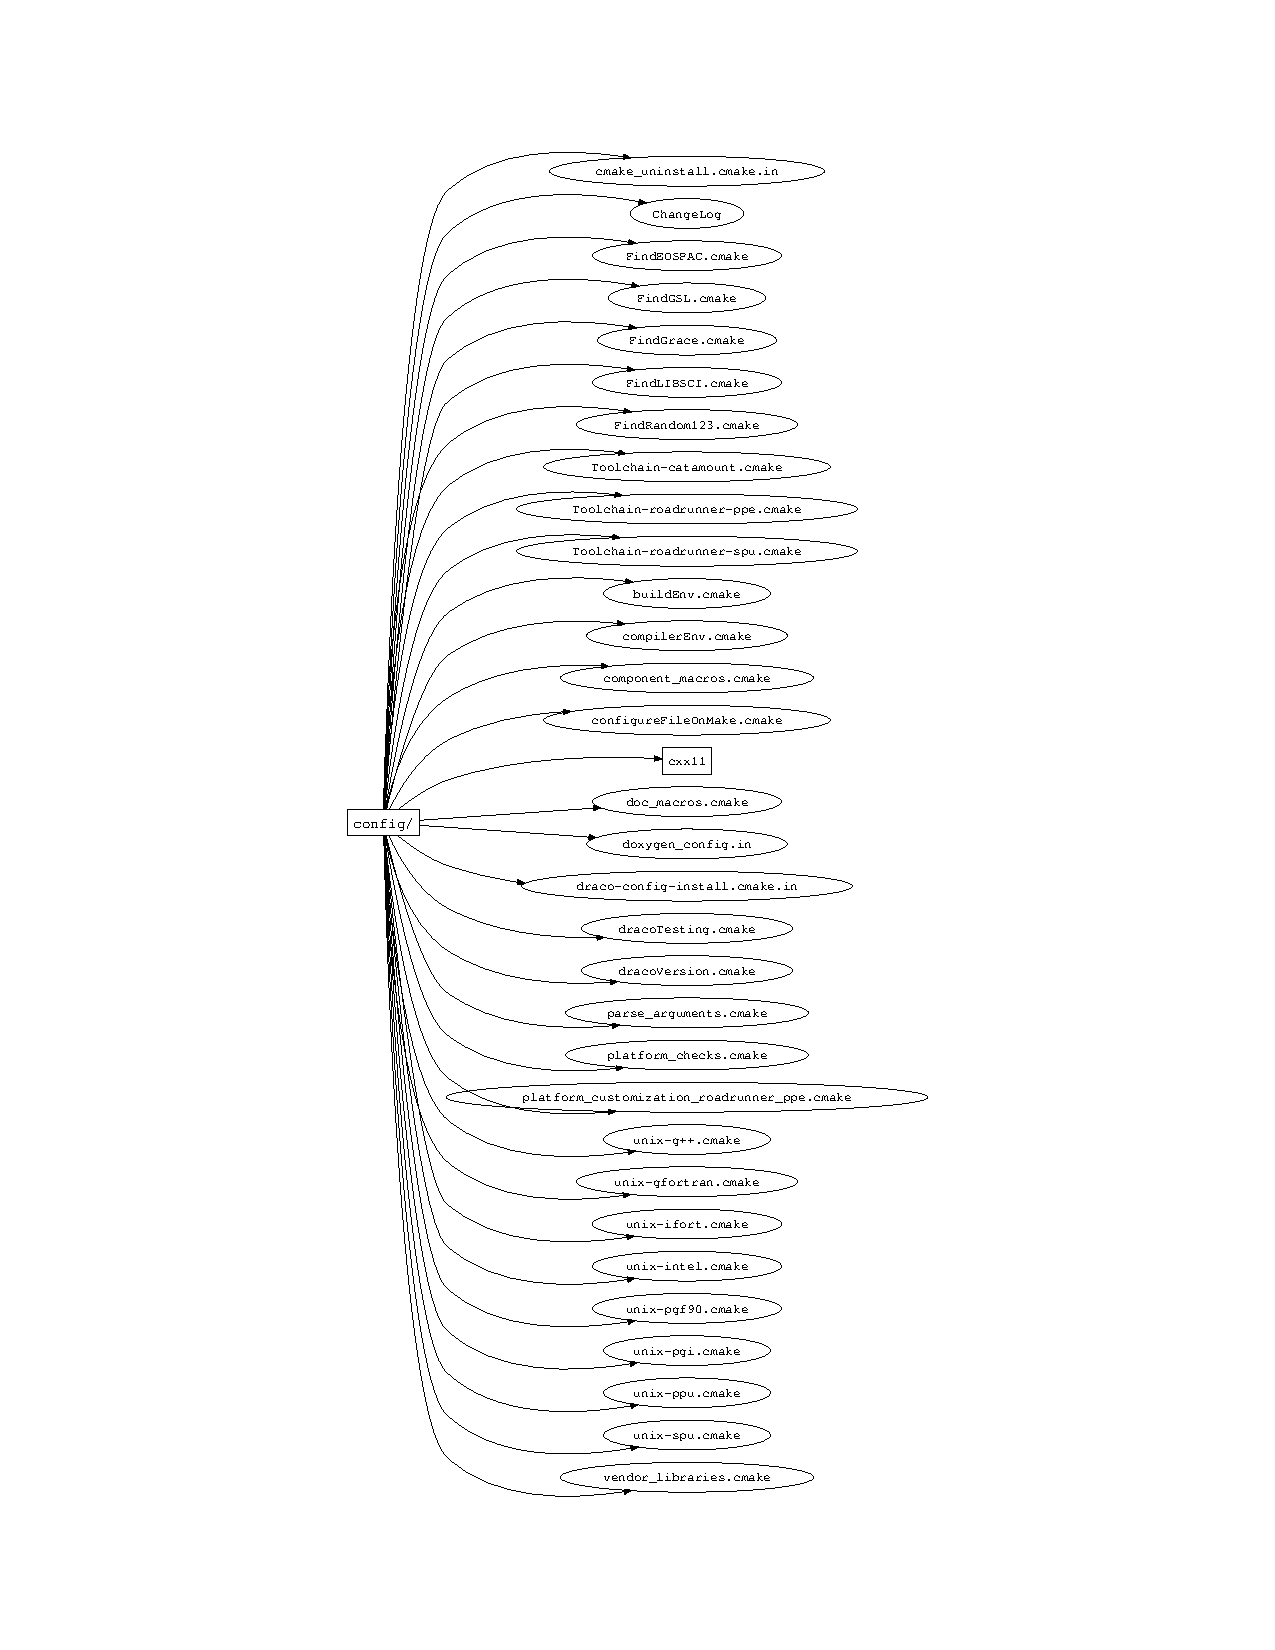
\includegraphics[clip,trim=4cm 2cm 10cm 0cm,width=2.0in]{fig/src_config}} 
      % \subfloat[\comp{tools/}]{\includegraphics[width=1.25in]{fig/src_tools.eps}} 
      \\
    \end{tabular}
  \end{center}
  \caption{Subdirectories under \comp{draco/}.  Directories are in
    boxes and files are in ellipses.}
  \label{fig:subdraco}
\end{figure}
complete source tree.
% not all directories under \comp{src/} will be released under certain \cvs\ checkouts.  
% The file \comp{draco\_config*} is a configure script that sets the proper paths to run configure in external directories.  
Under \draco\ there exists several files generated or needed by \cmake\ and \ctest.  The files \comp{CTestConfig.cmake} and \comp{CTestCustom.cmake} are read by \ctest\ and specify the location of the \draco\ dashboard and configuration setup for testing.  These settings include a list of source to omit from code coverage, tests to omit from dynamic analysis, warnings that should be ignored, etc.  The \comp{CMakeLists.txt} file is the primary build system configuration file parsed by \cmake\ in order to generate the build project (i.e.: Makefiles, project files, etc.).  The \comp{CMakeCache.txt} file is a template that developers can copy to their build sandbox and update initial build configuration settings before the first invocation of \cmake.  This file is not required by the \draco\ build system and is provided only as an aid for developers.
The \comp{*.cmake} files from the \comp{config} directory 
contains macro tests for configuring \draco.  Descriptions
of these files are given in Chap.~\ref{chap:extend}.  Finally, the
files \comp{Copyright}, \comp{ChangeLog}, and \comp{README.draco} are
descriptive ASCII files.

In the \comp{src/} directory there is a \comp{CMakeLists.txt} file that
instructs \cmake\ to setup the selected project generator, configure compiler options, run platform checks, locate and check vendor libraries, and tells \cmake\ to descend into each of the component directories for individual configuration. This file instructs \cmake\ to establish most of the build parameters and the master structure and inter-component dependencies.  The encapsulation and levelization of packages is controlled at this level.

In addition to the source code (\comp{.cc}, \comp{.hh}, and \comp{.h}
files), each component directory contains two build system files: 
A \comp{CMakeLists.txt} file controls the specific build instructions for the individual component including a list of sources to be compiled into a library.  The \comp{config.h.in} may not be provided with every component, but when it is provided it encapsulates preprocessor macro settings that are needed by the component.  Ref~\cite{autoconf} provides some background information on how the \comp{config.h.in} should be used.  Detailed discussions about how these files are used in \draco\ are given in Chaps.~\ref{chap:compile} and \ref{chap:adding}.

%In addition, each package directory may contain special files
%corresponding to the following formats
%\begin{verbatim}
%     <pkg>_<vendor>.h.in
%     Makefile.target
%     Makefile.srcs
%     Makefile.misc
%\end{verbatim}
%These files are used for special package configurations.  The file,
%\comp{<pkg>\_<vendor>.h.in}, is used to include vendor libraries that
%may not be installed in the standard \comp{\#include} and
%\comp{LD\_LIBRARY\_PATH} paths.  Details about the purpose of these
%files and their contents are given in Chaps.~\ref{chap:compile} and
%\ref{chap:adding}. 

Finally, each directory under \comp{src/} may contain source
subdirectories, \comp{doc/} subdirectories and \comp{autodoc} directories and should contain a \comp{test/} directory.  The
\comp{test/} directory holds component tests for the package.  Details
on how to compile the test directory using \ctest\ are given
in Chap.~\ref{chap:compile}.  Directions showing how to format
different test directories are given in Chap.~\ref{chap:adding}.

% ------------------------------------------ %
\subsection{Binary Directory Trees}

The \draco\ source is normally compiled in a separate, user-generated directory
tree called the \latin{target} or \latin{binary} directory tree\footnote{The GNU model normally uses the term \latin{target} directory while the \cmake\ community uses the term \latin{binary} directory, e.g.: \comp{PROJECT\_BINARY\_DIR}.}.  \index{binary directory} \index{target directory}  In this standard build mode, no files are
actually generated in the \draco\ source tree.  The \draco\ build system also supports building from within the source tree, but this mode of development is not recommended except in special circumstances (e.g: \soft{Eclipse} based projects work better when the source and binary tree are collocated). 

To configure \draco,
the user checks out a version of the source from \svn.  The checkout location is known as the \latin{source} directory.  In the \latin{binary} directory tree, the user runs \cmake\ with appropriate configure options.  These options can be provided (1) on the command line, (2) through the \cmake\ graphical interface via \comp{ccmake} \index{ccmake} or \comp{cmake-gui} \index{cmake-gui} or (3) by providing options in a \comp{CMakeCache.txt} \index{CMakeCache.txt} file located in the \latin{binary} directory.  \cmake\ will generate a directory tree
that is parallel to the \draco\ source tree with the appropriate
project and configuration files (e.g.: \comp{Makefile}, \comp{config.h}, \comp{draco.sln}, \comp{.project}, etc.).  Once the project files have been generated by \cmake, the compilation step can be initiated.  For a \latin{Unix Makefiles} based project this is accomplished by running \gmake\ from within the \latin{binary} directory.  The product of the compilation step is the generation of component libraries and executables by the selected compilers.  For non-\latin{Makefile} based projects, the \comp{all} or \comp{ALL\_BUILD} project target should be selected to begin compilation.

%In addition, \gmake\ installs the necessary \comp{.hh} and \comp{.h}
%files in a generated \comp{include/} directory.  Libraries are
%installed in a generated \comp{lib/} directory.  The \comp{include/}
%and \comp{lib/} directory locations are specified by the
%\comp{--prefix} tag in \autoconf.

For example, consider a parallel (MPI), debug configuration of \draco\ on a x86\_64 Linux
platform using the \soft{gcc} compiler suite.  The user might create a \latin{target} directory called
\comp{gcc\_mpid} and a \latin{build} directory under the target directory called \comp{draco}. After running \cmake\ with the
appropriate options\footnote{By default, the build system will configure for a debug build.  If MPI can be found on the local system, the build system will automatically enable parallel (MPI) features. The compiler set is chosen based on the value of environment variables \comp{CC}, \comp{CXX} and \comp{FC}.  If these variables are not set the build system will use whatever compiler it can find.  For this example, the configuration command is '\comp{cmake -DCMAKE\_INSTALL\_PREFIX=.. \$draco\_src\_dir}'},
%  and \gmake, 
the directory structure illustrated in Fig.~\ref{fig:build_tree} is generated.
\begin{figure}
  \centerline{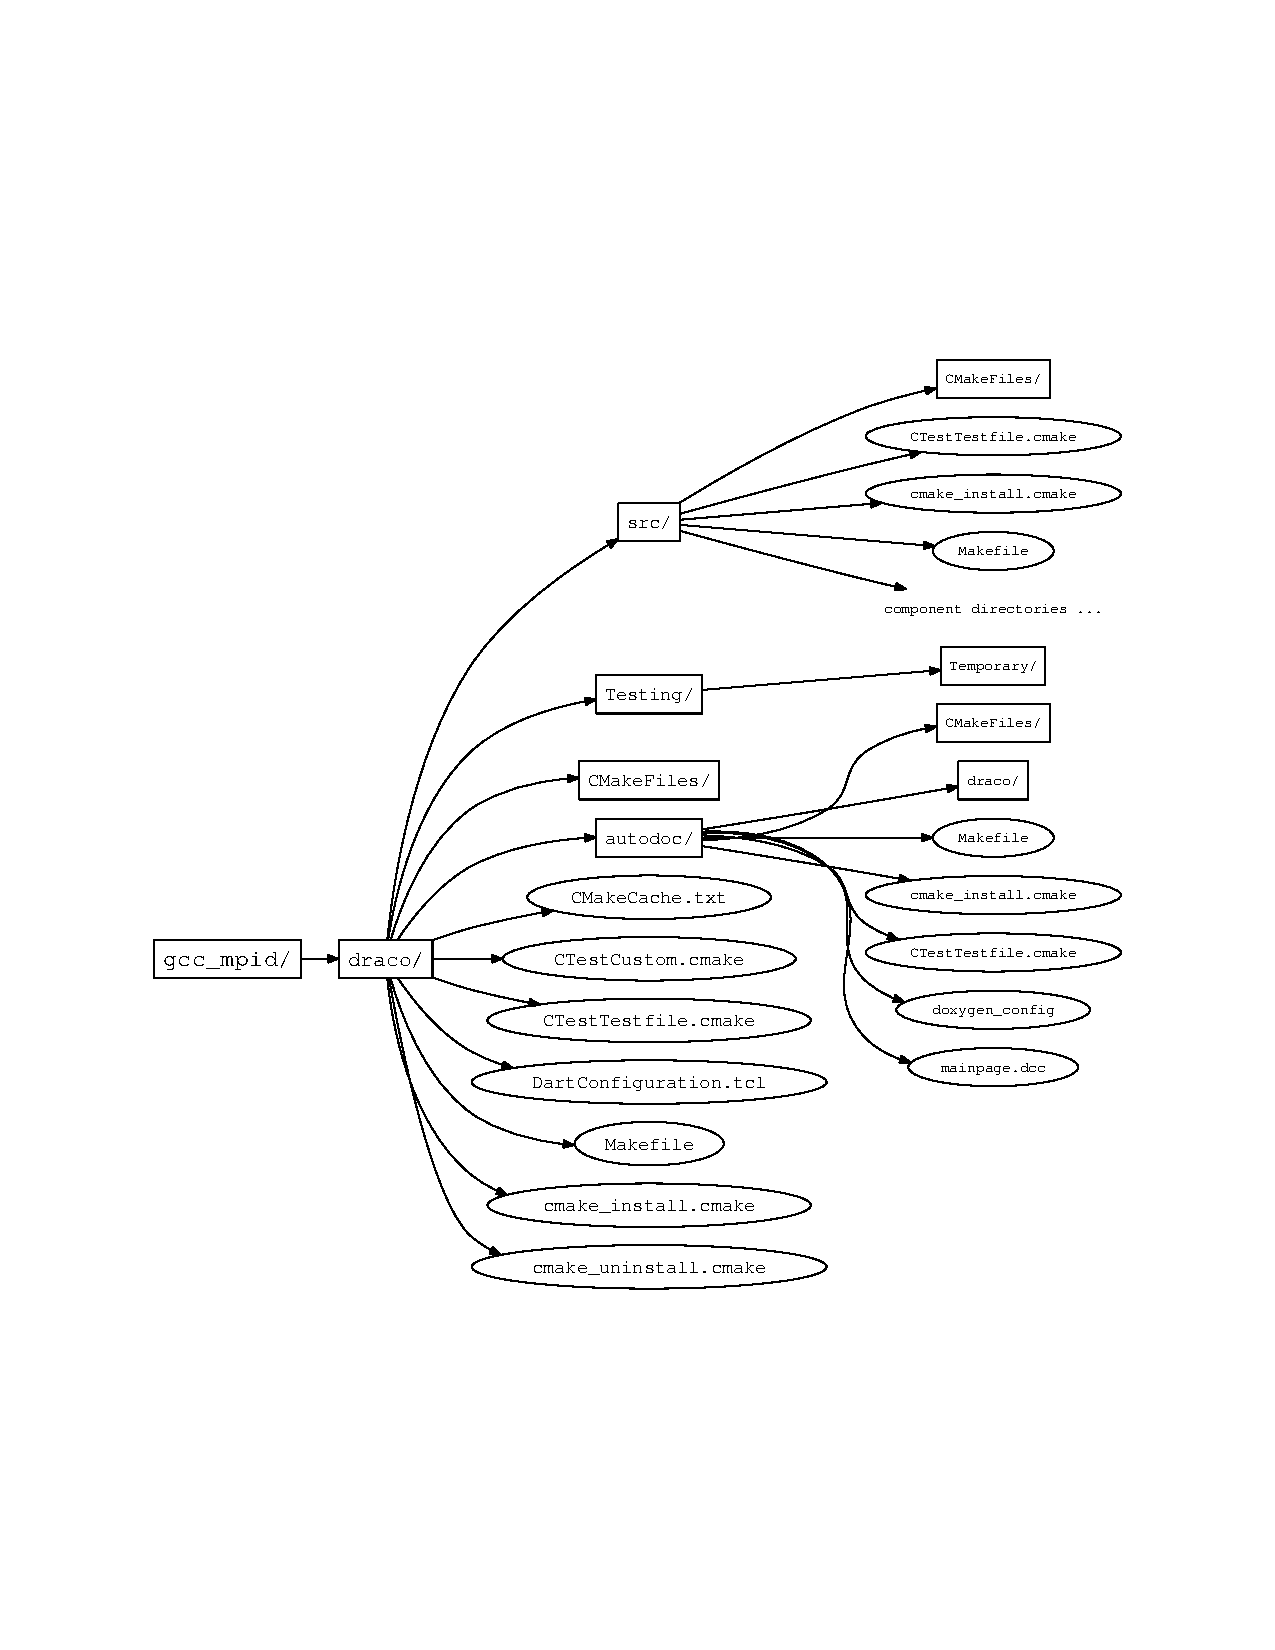
\includegraphics[width=6in]{fig/build_tree}}
  \caption{The \draco\ build tree after running \cmake\ for a Makefile-based project.  The \comp{source directories} are shown in
    Fig.~\ref{fig:subdraco}a. The \comp{doc directories} are shown in
    Fig.~\ref{fig:subdraco}b.}  The binary tree for \sys{Eclipse CDT4 - Unix Makefile} based projects will match this layout but will also include two additional dot files: \comp{.cproject} and \comp{.project}.
  \label{fig:build_tree}
\end{figure}
Inside of each component directory are Makefiles and configuration files
generated by \cmake.  Object (\comp{.o}) files are stored in the \comp{CMakeFiles/} directory along with specialized build and dependency instructions (\comp{depend.make}, \comp{flags.make}, \comp{link.txt}, etc.)
% Also, after building, the automatic
%dependency files (\comp{.cc.d} and \comp{.c.d}) will be found here
%along with the object (\comp{.o}) files.  

After building the project (possibly by running \make), the generated libraries and binary files will show up in the component directories.  The \draco\ build system is able to execute the compile step in parallel, utilizing all of the available local cores.  For \sys{Unix Makefile} based project, the option \comp{-j N} should be given to \make\ where the value of N is set to be the number of available cores on the local machine\footnote{Some developers have reported good results when requesting ~50\% more jobs than cores.  For example, for a machine that has 8 cores, the command \comp{make -j 12} has worked well.}.  \index{parallel make}

The generated files can be installed to the \latin{target} directory by building the \comp{install} target.  For development, it is a common practice to set the \latin{install} location to be the platform \latin{target} directory. \index{target directory} \index{install directory} This allows the generated libraries, headers and executable files to be stored under an appropriately named directory like \comp{gcc\_mpid} or \comp{intel10\_openmpi145\_rwdi} (Version 10 Intel compilers, OpenMPI version 1.4.5 and ReleaseWithDebInfo build model).  Running the \comp{install} target will add the \comp{lib/}, \comp{bin/}, \comp{include/} and \comp{config} directories under the  \latin{target} directory as shown in Figure~\ref{fig:build_tree_post_install}.
\begin{figure}
  \centerline{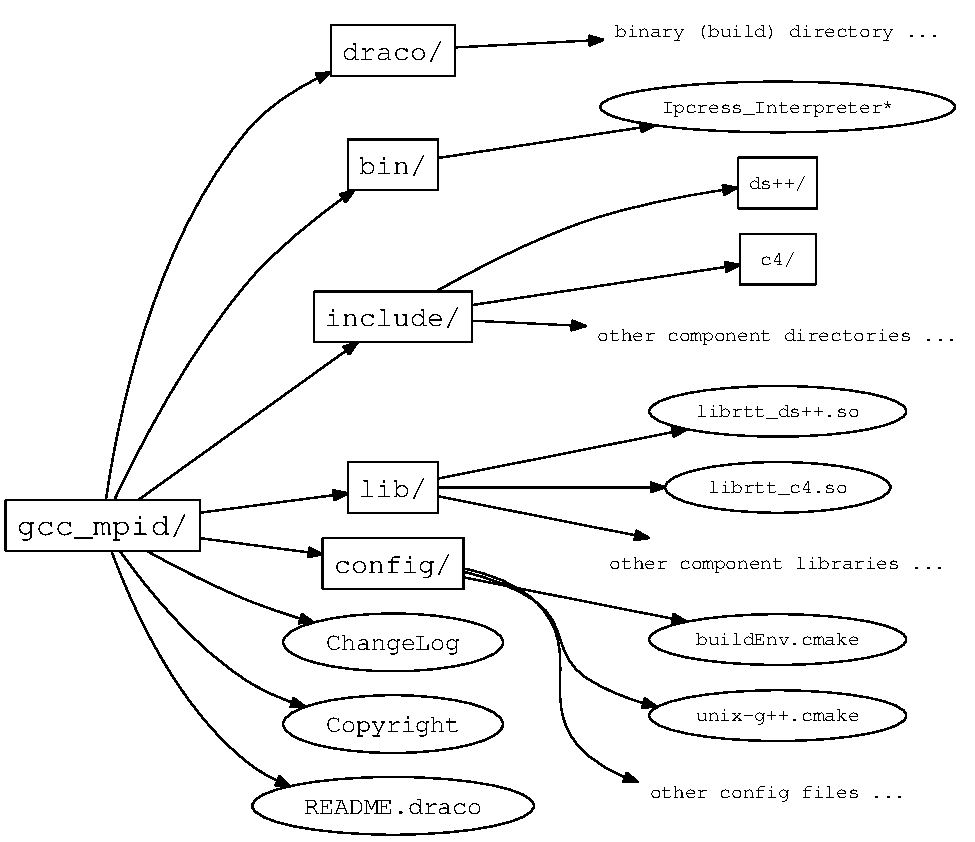
\includegraphics[width=6in]{fig/build_tree_post_install}}
  \caption{The \draco\ build tree after running \comp{make install} for a Makefile-based project.  The \latin{install} target creates  the \comp{lib/}, \comp{bin/}, \comp{include/} and \comp{config} directories under the  \latin{target} directory.  The target directory is specified at \latin{configure} time by setting the \cmake\ variable \comp{CMAKE\_INSTALL\_PREFIX}.}
  \label{fig:build_tree_post_install}
\end{figure}

%Appropriately, any files
%needed by a client system are found in the \comp{include/} and
%\comp{lib/} directories.  Also, multiple builds with different
%configuration options may be performed simultaneously.  All one has to
%do is generate a build directory for each configure.  

In many cases, \draco\ based software projects will be configured and compiled alongside \draco.  In this case, a binary directory for the client (e.g.: \clubimc\ or \capsaicin) might be found parallel to the \comp{draco} binary directory (see Fig.~\ref{fig:build_tree_post_install}) and the the client products (headers, libraries, etc.) are installed into the same target directory used by \draco.  Details on how to configure and compile \draco\ are found in Chap.~\ref{chap:compile}, \S~\ref{sec:configuring_draco} and \S~\ref{sec:building_draco}.


%%---------------------------------------------------------------------------%%

\section{Coding Conventions}
\label{sec:codeconventions}

\draco\ does not adhere strictly to any code convention for formatting, but it is recommended that developers attempt to follow the styles already used in existing source code.  The following subsections list specific code conventions that are required by \draco.

\subsection{File Extensions}
\label{sec:cc-fileext}

Table~\ref{tab:fileext} lists file extension standards used by \draco\ along with a description of the expected content type.
%
\begin{table}
  \begin{center}
    \caption{Draco Coding Conventions: Standard File Extensions}
    \label{tab:fileext}
    \begin{tabular}{p{0.5in}p{2.0in}p{3.5in}}\hline\hline
    
    File Extension & Description & Details \\ \hline
    \comp{.h} & ANSI C header file & Rarely used in \draco\ except for wrapping calls to vendor functions. \\
    \comp{.c} & ANSI C implementation file & Rarely used in \draco\ except for wrapping calls to vendor functions. \\
    \comp{.hh} & C++ declarations file & Common file that provide class and function declarations, including templated functions and classes.\\  
    \comp{.i.hh} & C++ inline implementation file & C++ implementation instructions that could be placed directly in the \comp{.hh} file.  These implementations are for inlined functions or implicitly instantiated template functions.  This file is always included directly by the \comp{.hh} file after all declarations have been made. \\
    \comp{.t.hh} & C++ template implementation file & C++ implementation instructions for explicitly instantiated functions.  This file always includes the associated \comp{.hh} file and is only included by an explicit instantiation file(\comp{\_pt.cc}). \\
    \comp{.cc} & C++ implementation file & C++ implementation instructions for functions declared in the \comp{.hh} file that are not to be inlined and are not template functions. \\
    \comp{\_pt.cc} & C++ explicit instantiation file & C++ explicit instantiations of templated classes and functions found in the associated declarations file. \\
    \comp{.in} & Files that must be processed & Usually found as \comp{config.h.in} that is processed into \comp{config.h} and provides preprocessor definitions used by the local component. \\
    \comp{.cmake} & \cmake\ build system file & Additional build system commands that have been extracted form \comp{CMakeLists.txt} files to improve reuse via cmake-macros. \\
	\hline \hline

    \end{tabular}
  \end{center}
\end{table}


\subsection{Tabs and editor width}
\label{sec:cc-tabs}

\draco\ developers have found that code is most cleanly viewed on various editors if spaces are used in place of tabs and the maximum column width is restricted to 80 columns.

%%---------------------------------------------------------------------------%%

\section{Summary}

In this chapter we have summarized the basic structure of the \draco\ 
build system.  We have illustrated the requirements for the \draco\ 
build system.  In the following chapters we will elaborate on the
details of how to configure, build, and test \draco\ installations.



%%---------------------------------------------------------------------------%%
%% ENDGAME
%%---------------------------------------------------------------------------%%

\bibliographystyle{rnote}
\bibliography{../bib/draco}

\printindex

\closing
\end{document}

%%---------------------------------------------------------------------------%%
%% end of dbs.tex
%%---------------------------------------------------------------------------%%
